\documentclass[11pt,nocut]{article}

\usepackage{../latex_style/packages}
\usepackage{../latex_style/notations}
%\externaldocument{../lecture_02/lecture_02}
\externaldocument{../lecture_07/lecture_07}


\title{\vspace{-2.0cm}%
	Optimization and Computational Linear Algebra for Data Science\\
Lecture 10: Optimality conditions}
\author{Léo \textsc{Miolane} \ $\cdot$ \ \texttt{leo.miolane@gmail.com}}
\date{\today}

\begin{document}
\maketitle
\textbf{Warning:}
\emph{This material is not meant to be lecture notes. It only gathers the main concepts and results from the lecture, without any additional explanation, motivation, examples, figures...
}


\section{Local and global minimizers}

We aim at minimizing a function $f: \R^n \to \R$.
We say that $x^* \in \R^n$ is
\begin{itemize}
	\item a \emph{global} minimizer of $f$ if for all $x \in \R^n$, $f(x^*) \leq f(x)$.
	\item a \emph{local} minimizer of $f$ if there exists $\delta > 0$ such that for all $x \in B(x^*,\delta)$, $f(x^*) \leq f(x)$.
\end{itemize}
Of course, a global minimizer if also a local minimizer but the converse is not true.

\begin{proposition}\label{prop:zero_grad}
	Let $x \in \R^n$ be a point at which $f$ is differentiable. 
	Then
	$$
	x \ \text{is a local minimizer of} \ f \ \implies \nabla f(x) = 0.
	$$
\end{proposition}

If $f$ is convex then the converse is true:

\begin{proposition}\label{prop:zero_grad_convex}
	Assume that $f$ is convex.
	Let $x \in \R^n$ be a point at which $f$ is differentiable. 
	Then
	$$
	\nabla f(x) = 0 \ \implies \ x \ \text{is a global minimizer of} \ f.
	$$
\end{proposition}

\section{Constrained optimization}

We would now like to investigate constrained optimization problems:
\begin{equation}\label{eq:problem}
	\begin{array}{lll}
		\text{minimize} & f(x) & \\
		\text{subject to} & g_i(x) \leq 0, & i=1, \dots, m \\
						  & h_i(x) = 0, & i=1, \dots, p,
	\end{array}
\end{equation}
with variable $x \in \R^n$.
Here we have $m$ inequality constraints $g_1(x) \leq 0, \dots, g_m(x)\leq  0$ and $p$ equality constraints $h_1(x) = 0, \dots, h_p(x) = 0$ to satisfy.
We denote by $p^* \in \R \cup \{\pm \infty\}$ the optimal value of \eqref{eq:problem}.

\begin{definition}[Feasible point]
	A point $x \in \R^n$ is \emph{feasible} if it satisfies all the constraints: $g_1(x) \leq 0, \dots, g_m(x)\leq  0$ and $h_1(x) = 0, \dots, h_p(x) = 0$. We will denote by $F$ the set of feasible points.
\end{definition}

\begin{definition}[Active constraints]
	We say that the inequality constraint $g_i(x) \leq 0$ is active at $x$ if $g_i(x) = 0$.
	We let $\mathcal{A}(x)$ be the set of active constraints at $x$: $\mathcal{A}(x) = \{ i \, | \, g_i(x) = 0\}$.
\end{definition}
We would now get for the problem \eqref{eq:problem} the analog of Proposition \ref{prop:zero_grad}.
Since an equality constraint $h_i(x) = 0$ can be equivalently written in two inequality constraints $h_i(x) \leq 0$ and $-h_i(x) \leq 0$, we can assume to have only inequality constraints.
For simplicity, we first assume to have only one inequality constraint $g(x) \leq 0$ so that \eqref{eq:problem} reduces to
\begin{equation}\label{eq:problem2}
	\text{minimize} \ f(x) \ \text{subject to} \ g(x) \leq 0.
\end{equation}


Let $x$ be a solution of \eqref{eq:problem2}, i.e.\ $g(x) \leq 0$ and $f(x) \leq f(x')$ for all $x'$ such that $g(x')\leq0$
We distinguish two cases:

\paragraph{Case 1: the constraint is not active at $x$; $g(x) <0$.} In that case $x$ is in the interior of $F$: one can find $\delta > 0$ such that $B(x,\delta) \subset F$. Since $x$ is a solution of \eqref{eq:problem2} we have for all $x' \in B(0,\delta)$, $f(x) \leq f(x')$. One can therefore apply Proposition \ref{prop:zero_grad} to get that $\nabla f(x) = 0$.

We conclude that in the case where the constraint is not active, the constraint does not play any role and one gets the same optimality condition as in the unconstrained setting.

\paragraph{Case 2: the constraint is active at $x$; $g(x) = 0$.}
In that case, there exists $\lambda \geq 0$ such that 
\begin{equation}\label{eq:grad_active}
	\nabla f(x) = - \lambda \nabla g(x).
\end{equation}
To see that, assume that \eqref{eq:grad_active} does not hold. Then we are in the following situation:
\begin{figure}[h!]
	\begin{center}
		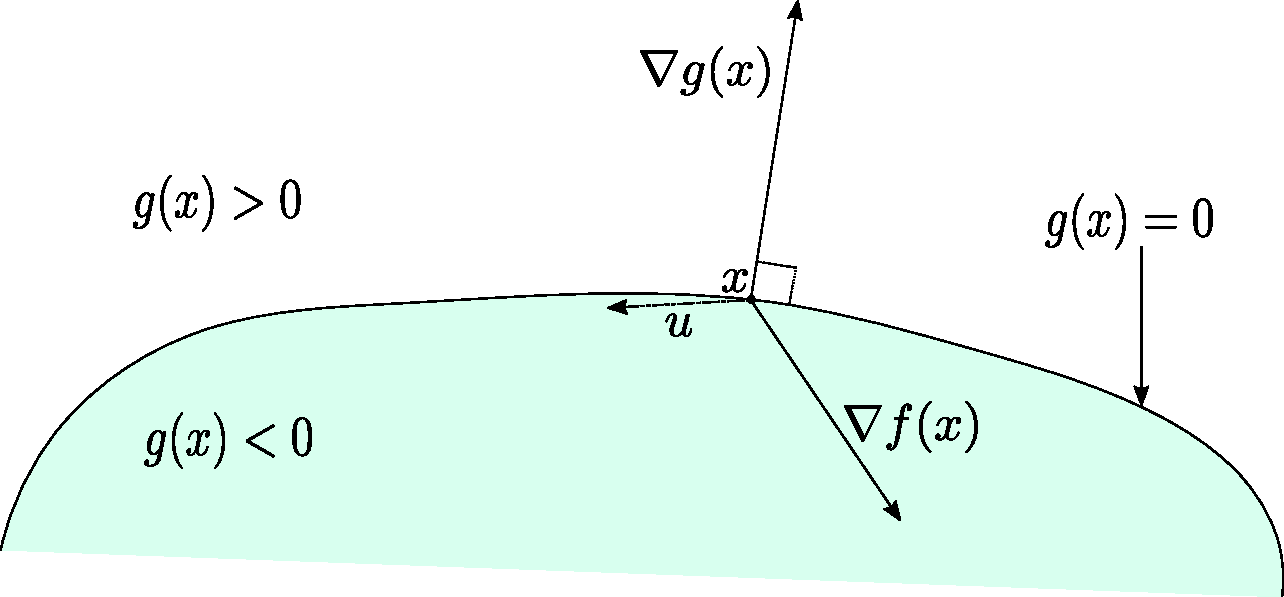
\includegraphics[width=0.8\linewidth]{figures/absurd.pdf}
	\end{center}
\end{figure}

As we can see on the figure, we can find a vector $u$ such that
$$
\langle u, \nabla g(x) \rangle < 0 
\quad \text{and} \quad
\langle u, \nabla f(x) \rangle < 0.
$$
Starting from $x$ and following the direction $u$ one remains in the feasible set because for small $\delta >0$
$$
g(x + \delta u) \simeq g(x) + \delta \langle u, \nabla g(x) \rangle \leq 0.
$$
Moreover, $f$ decreases locally on the direction $u$:
$$
f(x + \delta u) \simeq f(x) + \delta \langle u, \nabla f(x) \rangle < f(x).
$$
This means that one can find $\delta > 0$ such that $x + \delta u$ is feasible and such that $f(x + \delta u) < f(x)$. This contradicts the assumption that $x$ is solution of \eqref{eq:problem2}.
We conclude that \eqref{eq:grad_active} holds, i.e.\ that there exists $\lambda \geq 0$ such that
$$
\nabla f(x) + \lambda \nabla g(x) = 0.
$$

We will only cover the case where the equality constraints are linear, i.e. $h_i(x) = \langle a_i, x \rangle + b_i$ for from $a_i \in \R^n$ and $b_i \in \R$.

This generalize to the case \eqref{eq:problem} where we have multiple constraints:

\begin{definition}[LICQ]
	Let $x$ be a feasible point. We say that the \emph{linear independence constraint qualification} (LICQ) holds at $x$ if the set of gradients
	$$
	\big\{ \nabla g_i(x) \, \big| \, i \in \mathcal{A}(x) \big\}
	\cup
	\big\{ \nabla h_i(x) \, \big| \, i \in \{1, \dots, p\} \big\}
	$$
	is linearly independent.
\end{definition}

\begin{theorem}[First-order optimality conditions]\label{th:first_order}
	Assume that the functions $f$, $g_1, \dots, g_m$ are continuously differentiable and that $h_1, \dots, h_p$ are linear. If $x$ is solution of \eqref{eq:problem} and if LICQ holds at $x$
	then there exists $\lambda_1, \dots, \lambda_m \geq 0$ and $\nu_1, \dots, \nu_p \in \R$ such that:
	\begin{equation}\label{eq:kkt}
		\nabla f(x) + \sum_{i=1}^m \lambda_i \nabla g_i(x) + \sum_{i=1}^p \nu_i \nabla h_i(x) = 0.
	\end{equation}
	Moreover $\lambda_i = 0$ if $g_i(x) < 0$.
\end{theorem}

The scalars $\lambda_i, \nu_i$ are called \emph{Lagrange multipliers}.
The first-order conditions of Theorem \ref{th:first_order} are often called the Karush-Kuhn-Tucker (KKT) conditions and Theorem \ref{th:first_order} is presented the following way.
If $x$ is a solution of \eqref{eq:problem} then there exists numbers $\lambda_i,\nu_i$ such that:
\begin{enumerate}[label=(\roman*)]
	\item\label{item:kkt1} \emph{Primal feasibility}: $g_i(x) \leq 0$ for $i=1, \dots, m$ and $h_i(x) = 0$ for $i=1, \dots, p$.
	\item\label{item:kkt2} \emph{Dual feasibility}: $\lambda_i \geq 0$ for $i=1, \dots, m$.
	\item\label{item:kkt3} \emph{Stationarity}: $\nabla f(x) + \sum\limits_{i=1}^m \lambda_i \nabla g_i(x) + \sum\limits_{i=1}^p \nu_i \nabla h_i(x) = 0$.
	\item\label{item:kkt4} \emph{Complementary slackness}: $\lambda_i g_i(x) = 0$ for $i = 1 ,\dots, m$.
\end{enumerate}
The terms ``primal'' and ``dual'' will be explained in the next section.

\section{The Lagrangian and the dual problem}

We define the Lagrange dual function $L$ associated with the problem \eqref{eq:problem} by
\begin{equation}
	L(x,\lambda,\nu) = 
	f(x) + \sum_{i=1}^m \lambda_i g_i(x) + \sum_{i=1}^p \nu_i h_i(x),
\end{equation}
where $x \in \R^n$, $\lambda \in \R_{\geq 0}^m$ and $\nu \in \R^p$. We define the Lagrange dual function by
$$
\ell(\lambda,\nu) = \inf_{x \in \R^n} L(x,\lambda,\nu).
$$
Notice that for all feasible point $x$,
$$
L(x,\lambda,\nu)
= f(x) + \sum_{i=1}^m \lambda_i g_i(x) \leq f(x)
$$
because $h_i(x) = 0$ and $\lambda_i g_i(x) \leq 0$. By taking the infimum in $x$ on both sides of the inequality we get a lower bound on the value of the optimization problem \eqref{eq:problem}:
\begin{proposition}
	%Let $p^*$ be the optimal value of the problem \eqref{eq:problem}.
	For all $\lambda_1, \dots, \lambda_m \geq 0$ and all $\nu_1, \dots,\nu_p \in \R$ we have:
	\begin{equation}\label{eq:dual_lower_bound}
		\ell(\lambda,\nu) \leq p^*.
	\end{equation}
\end{proposition}

\subsection{Dual problem}

We would like to make the lower bound \eqref{eq:dual_lower_bound} as tight as possible: one would like therefore to solve the so-called \emph{dual problem}:
\begin{equation}\label{eq:dual_problem}
	\begin{array}{lll}
		\text{maximize} & \ell(\lambda,\nu) & \\
		\text{subject to} & \lambda_i \geq 0, & i=1, \dots, m \\
						  & \nu_i \in \R, & i=1, \dots, p.
	\end{array}
\end{equation}
Notice that the Lagrange dual function is always concave, as an infimum of linear functions. Hence, the dual problem might be easier to solve than the original problem.
\\

We denote by $d^*$ the optimal value of the dual problem \eqref{eq:dual_problem}.
From \eqref{eq:dual_lower_bound} we deduce that the optimal value of the primal problem is greater or equal than the one of the dual problem:
\begin{equation}\label{eq:weak_duality}
	d^* \leq p^*.
\end{equation}
This is known as \emph{weak duality}.
Notice that $p^* = \inf_{x \in \R^n} F(x)$ where
$$
F(x) \defeq
\sup_{\lambda \geq 0, \nu} L(x,\lambda,\nu)
=
\begin{cases}
	f(x) & \text{if} \ x \ \text{is feasible},\\
	+ \infty & \text{otherwise.}
\end{cases}
$$
Hence, the weak duality inequality can be rewritten as:
\begin{equation}\label{eq:sup_inf}
	\sup_{\lambda \geq 0, \nu} \inf_{x \in \R^n} L(x,\lambda,\nu) \leq \inf_{x \in \R^n} \sup_{\lambda \geq 0, \nu} L(x,\lambda,\nu).
\end{equation}

When there is equality in \eqref{eq:weak_duality} (or equivalently in \eqref{eq:sup_inf}) we say that there is \emph{strong duality}. We will see in the next section that strong duality holds for convex problems under mild assumptions.


\subsection{Saddle-points}
\begin{definition}[Saddle-point]
	We say that $(x; \lambda,\nu) \in \R^n \times \R_{\geq 0}^m \times \R^p$ is a \emph{saddle-point} of $L$ if
	\begin{equation}\label{eq:def_saddle}
	\forall (\lambda',\nu') \in \R_{\geq 0}^m \times \R^p \quad
	L(x,\lambda',\nu') \leq L(x,\lambda,\nu) \leq L(x',\lambda,\nu) \quad \forall x' \in \R^n.
\end{equation}
\end{definition}

Notice that if $(x; \lambda,\nu)$ is a saddle-point of $L$, then $x$ is solution of \eqref{eq:problem}. Indeed, by taking the supremum over $(\lambda',\nu')$ in \eqref{eq:def_saddle} we get:
$$
F(x) \leq L(x,\lambda,\nu) \leq L(x',\lambda,\nu) \leq F(x')
$$
for all $x' \in \R^n$. 
This gives that $F(x) = \min F = L(x,\lambda,\nu)$.
By a ``symmetric'' argument one also gets that $(\lambda,\nu)$ is a solution of the dual problem \eqref{eq:dual_problem} and $\ell(\lambda,\nu) = \max_{\lambda \geq 0,\nu} \ell(\lambda',\nu') = L(x,\lambda,\nu)$.

We conclude that if $(x,\lambda,\nu)$ is a saddle-point of $L$, then $x$ is primal optimal, that $(\lambda,\nu)$ is dual optimal and that strong duality holds. The next Theorem shows that the converse is true.

\begin{theorem}\label{th:saddle}
	Let $(x; \lambda,\nu) \in \R^n \times \R_{\geq 0}^m \times \R^p$. Then
	\vspace{-4mm}
	$$
	(x;\lambda,\nu) \ \text{is a saddle-point of} \ L
	\quad \Longleftrightarrow \quad
	\begin{cases}
x \ \text{is a solution of the primal problem} \ \eqref{eq:problem}, \\
(\lambda,\nu) \ \text{is a solution of the dual problem} \ \eqref{eq:dual_problem}, \\
	\text{strong duality holds.}
	\end{cases}
	$$
	\vspace{-3mm}
\end{theorem}
	%\begin{equation}\label{eq:th_saddle}
	%F(x)
	%= 
	%\inf_{x'}\sup_{\lambda' \geq 0, \nu'} L(x',\lambda',\nu')
	%=
	%\sup_{\lambda' \geq 0, \nu'}
	%\inf_{x'}
	%L(x',\lambda',\nu') 
	%= \ell(\lambda,\nu),
	%\end{equation}
	%i.e.\ if and only if 
\begin{proof}
Assume that $x$ is a solution of the primal problem \eqref{eq:problem}, that $(\lambda,\nu)$ is a solution of the dual problem \eqref{eq:dual_problem} and strong duality holds.
We have
$$
\ell(\lambda,\nu) = \inf_{x'} L(x',\lambda,\nu) \leq
L(x,\lambda,\nu) \leq \sup_{\lambda' \geq 0, \nu'} L(x,\lambda',\nu') = F(x).
$$
Since there is strong duality, we have $\ell(\lambda,\nu) = F(x)$: hence the inequalities above are in fact equalities. This implies that $(x;\lambda,\nu)$ is a saddle-point of $L$.
\end{proof}

\subsection{Solving the primal problem via the dual}

Assume that strong duality holds and that we have found a solution $(\lambda^*,\nu^*)$ of the dual problem. 
By Theorem \ref{th:saddle} we get that a point $x^* \in \R^n$ is a solution of the primal problem if and only if $(x^*;\lambda^*,\nu^*)$ is a saddle-point of $L$:
$$
x^* \quad \text{is solution of the primal problem} \quad
\Longleftrightarrow
\quad
\left\{
	\!\!
\begin{array}{lll}
	x^* & \text{minimizes} & L(\cdot, \lambda^*,\nu^*), \\
	(\lambda^*,\nu^*) & \text{maximizes} & L(x^*, \cdot, \cdot).
\end{array}
\right.
$$
Notice that $(\lambda^*,\nu^*)$ maximizes the linear function $L(x^*, \cdot,\cdot)$ if and only if $x^*$ is feasible. We obtain:
$$
x^* \quad \text{is solution of the primal problem} \quad
\Longleftrightarrow
\quad
\begin{cases}
	x^* \quad \text{minimizes} \quad L(\cdot, \lambda^*,\nu^*), \\
	x^* \quad \text{is feasible.}
\end{cases}
$$

This is particularly useful, because the dual problem might be easier to solve than the primal one. In the case when there is strong duality, the equivalence above tells us that it suffices then to solve the \textbf{unconstrained} optimization problem $\min_{x \in \R^n} L(x,\lambda^*,\nu^*)$.
Assume for simplicity that $x \mapsto L(x,\lambda^*,\nu^*)$ admits a unique minimizer $x^*$. Then if $x^*$ is feasible then it is a solution of the problem \eqref{eq:problem}. 
If $x^*$ is not feasible then the minimum of \eqref{eq:problem} can not be attained.

\section{Kuhn Tucker Theorem}

In this section, we assume that the functions $f$, $g_1, \dots, g_m$ are convex and that $h_1, \dots, h_p$ are linear. We say then that the optimization problem \eqref{eq:problem} is convex.
Notice in that case that the set of feasible points is convex, as the intersection of the convex sets $\{x | g_i(x) \leq 0 \}$ and $\{x|h_i(x) =0\}$.
\\

We will see in this section that \textbf{strong duality holds for convex problems under mild assumptions}, known as ``Slater's condition''.


\begin{definition}[Slater's condition]
	We say that the problem \eqref{eq:problem} verifies Slater's condition if there exists a feasible point $x$ such that $g_i(x) < 0$ for all $i \in \{1, \dots, m\}$.
\end{definition}

\begin{proposition}\label{prop:slater}
	If the problem \eqref{eq:problem} is convex and verifies Slater's condition, then strong duality holds and the optimal value of the dual problem is attained at some $(\lambda,\nu) \in \R_{\geq 0}^m \times \R^p$.
\end{proposition}
We refer to Section~5.2.3 of~\cite{boyd2004convex} for a proof of Proposition \ref{prop:slater}.



\begin{theorem}[Kuhn Tucker]\label{th:kuhn_tucker}
	Assume that the functions $f$, $g_1, \dots, g_m$ are \textbf{convex}, differentiable and that $h_1, \dots, h_p$ are linear. Assume that strong duality holds and that the optimal value of the dual problem is attained at some $(\lambda,\nu) \in \R_{\geq 0}^m \times \R^p$. (This is for instance the case under Slater's condition).
	\\

	Then $x \in \R^n$ is solution of \eqref{eq:problem} if and only if $x$ is feasible and
	\begin{equation}\label{eq:kkt}
		\begin{cases}
			\displaystyle \nabla f(x) + \sum_{i=1}^m \lambda_i \nabla g_i(x) + \sum_{i=1}^p \nu_i \nabla h_i(x) = 0 \\
		\lambda_i g_i(x) = 0 \quad \text{for all} \quad i=1, \dots, m.
		\end{cases}
	\end{equation}
	In other words, a feasible point $x$ is a solution of \eqref{eq:problem} if and only if $(x; \lambda, \nu)$ is a saddle-point of the Lagrangian $L$.
\end{theorem}

\noindent Such couple $(\lambda,\nu)$ is sometimes called a ``dual certificate'', since it certifies the optimality of $x$.
\\

\begin{proof}[of Theorem \ref{th:kuhn_tucker}]
	Let $x$ be a feasible point.
	By Theorem \ref{th:saddle} we have
	\begin{center}
		$x$ solution of \eqref{eq:problem} $\Longleftrightarrow$ $(x; \lambda, \nu)$ is a saddle-point of the Lagrangian $L$.
	\end{center}
	
	We assumed that the problem \eqref{eq:problem} is convex. 
	The function $L(\cdot, \lambda,\nu)$ is thus convex and the function $L(x,\cdot,\cdot)$ is concave (in fact it is affine). Hence
	\begin{align*}
			\nabla f(x) + \sum_{i=1}^m \lambda_i \nabla g_i(x) + \sum_{i=1}^p \nu_i \nabla h_i(x) = 0
			\quad &\Longleftrightarrow \quad
			x \ \text{minimizes} \ L(\cdot,\lambda,\nu)
			\\
		\lambda_i g_i(x) = 0 \quad \text{for all} \quad i=1, \dots, m
		\quad &\Longleftrightarrow \quad
			(\lambda,\nu) \ \text{maximizes} \ L(x,\cdot,\cdot).
	\end{align*}
	We get that \eqref{eq:kkt} $\Longleftrightarrow$ $(x;\lambda,\nu)$ is a saddle-point of $L$, which concludes the proof.
\end{proof}

\section*{Further reading}

See Chapter 12 from \cite{nocedal2006numerical} for a proof of Theorem \ref{th:first_order}. See in particular section 12.6 for constraint qualifications that are more general than LICQ.
See Chapters 4 and 5 of \cite{boyd2004convex} a more detailed introduction to convex optimization problems and duality.

\vspace{1cm}
\centerline{\pgfornament[width=7cm]{71}}


\bibliographystyle{plain}
\bibliography{../references.bib}
\end{document}
